\documentclass{article}
\usepackage[utf8]{inputenc}
\usepackage{amsmath}
\usepackage{amssymb}
\usepackage{graphicx}

\begin{document}

\section*{Radioactive Decay}
For radioactive substances $A$ and $B$ consider the decay chain
\begin{equation*}
    A \overset{\lambda_{1}}{\longrightarrow} B \overset{\lambda_{2}}{\longrightarrow} C
\end{equation*}
$A$ decays into $B$ with a decay rate $\lambda_{1}$ and B decays into a third substance $C$ with decay rate $\lambda_{2}$. The evolution of the amounts $\Phi_{A}\left(t\right)$, $\Phi_{B}\left(t\right)$ of the substances $A$ and $B$ can be modelled by the following coupled system of ordinary differential equations
\begin{align}
    \frac{\mathrm{d}\Phi_{A}}{\mathrm{d} t}\left(t\right) &= -\lambda_{1}\Phi_{A}\left(t\right) \\
    \frac{\mathrm{d}\Phi_{B}}{\mathrm{d} t}\left(t\right) &= -\lambda_{2}\Phi_{B}\left(t\right) + \lambda_{1}\Phi_{A}\left(t\right)
\end{align}
\subsection*{8-11.a}
We are tasked with calculating the analytical solution of the above system using the method of variation of constants. We can solve equation (1) as it only depends on $\Phi_{A}\left(t\right)$. We rewrite the equation into the usual form using $y := \Phi_{A}$
\begin{equation*}
    y' = -\lambda_{1}y \implies y' +\lambda_{1}y = 0
\end{equation*}
which gives us a homogeneous linear ODE of first degree, we get the corresponding characteristic polynomial
\begin{equation*}
    \alpha + \lambda_{1} = 0 \implies \alpha = \lambda_{1}
\end{equation*}
and thus the solution
\begin{equation*}
    \Phi_{A}\left(t\right) = y = A_{0}e^{-\lambda_{1}t}
\end{equation*}
Let us plug this into the second equation, which yields
\begin{equation*}
    \frac{\mathrm{d}\Phi_{B}}{\mathrm{d} t}\left(t\right) = -\lambda_{2}\Phi_{B}\left(t\right) + \lambda_{1}A_{0}e^{-\lambda_{1}t}
\end{equation*}
which now is not dependent on $\Phi_{A}$ anymore and we can hence solve using the usual techniques. We will rewrite the system into the usual notation which makes computations a bit less tedious. We use the notation $y := \Phi_{B}$ and get
\begin{equation*}
    y' = -\lambda_{2}y + \lambda_{1}A_{0}e^{-\lambda_{1}t} \Longleftrightarrow y' +\lambda_{2}y =  \lambda_{1}A_{0}e^{-\lambda_{1}t}
\end{equation*}
This is a linear differential equation of order $1$, which we can again solve in two parts. We first solve the homogeneous equation
\begin{equation*}
    y' + \lambda_{2}\lambda_{1} = 0 
\end{equation*}
for which we get the homogeneous equation $\alpha + \lambda_{2} = 0$ and thus $\alpha = -\lambda_{2}$, which yields the homogeneous solution
\begin{equation*}
    y_{h} = B_{0}e^{-\lambda_{2}t}
\end{equation*}
the inhomogeneous equation we solve using the variation of constants technique proposed by the exercise description. We assume here that the constant $B_{0}$ is itself a function of $t$ and that the particular solution will be of the form 
\begin{align*}
    y_{p} &= B_{0}\left(t\right)e^{-\lambda_{2}t} \\
    y_{p}' &= B_{0}'\left(t\right)e^{-\lambda_{2}t} - \lambda_{2}B_{0}\left(t\right)e^{-\lambda_{2}t} \quad \text{(product rule)}
\end{align*}
Putting this into our ODE yields
\begin{equation*}
    B_{0}'\left(t\right)e^{-\lambda_{2}t} \underbrace{\:- \lambda_{2}B_{0}\left(t\right)e^{-\lambda_{2}t} +\lambda_{2}B_{0}\left(t\right)e^{-\lambda_{2}t}\:}_{=0} =  \lambda_{1}A_{0}e^{-\lambda_{1}t} 
\end{equation*}
and hence 
\begin{equation*}
    B_{0}'\left(t\right)e^{-\lambda_{2}t} = \lambda_{1}A_{0}e^{-\lambda_{1}t} \implies B_{0}'\left(t\right) = \lambda_{1}A_{0}\frac{e^{-\lambda_{1}t}}{e^{-\lambda_{2}t}} = \lambda_{1}A_{0}e^{\left(\lambda_{2}-\lambda_{1}\right)t}
\end{equation*}
from this we get
\begin{equation*}
    \int B_{0}'\left(t\right) \mathrm{d}t = B_{0}\left(t\right) =  \lambda_{1}A_{0}\int e^{\left(\lambda_{2}-\lambda_{1}\right)t}\mathrm{d}t
\end{equation*}
Substitution with $u = \left(\lambda_{2}-\lambda_{1}\right)t$ giving $\mathrm{d}u = \left(\lambda_{2}-\lambda_{1}\right)\mathrm{d}t \implies \mathrm{d}t = \frac{1}{\lambda_{2}-\lambda_{1}}\mathrm{d}u$. Which then gives us
\begin{equation*}
    \lambda_{1}A_{0}\int e^{\left(\lambda_{2}-\lambda_{1}\right)t}\mathrm{d}t = \frac{\lambda_{1}A_{0}}{\lambda_{2}-\lambda_{1}}\int e^{u} \mathrm{d}u = \frac{\lambda_{1}A_{0}}{\lambda_{2}-\lambda_{1}} e^{u} = \frac{\lambda_{1}A_{0}}{\lambda_{2}-\lambda_{1}} e^{\left(\lambda_{2}-\lambda_{1}\right)t}
\end{equation*}
and hence the we get
\begin{equation*}
    B_{0}\left(t\right) = \frac{\lambda_{1}A_{0}}{\lambda_{2}-\lambda_{1}} e^{\left(\lambda_{2}-\lambda_{1}\right)t} = \frac{\lambda_{1}A_{0}}{\lambda_{2}-\lambda_{1}} \cdot\frac{e^{\lambda_{2}t}}{e^{\lambda_{1}t}} \implies y_{p} = \frac{\lambda_{1}A_{0}}{\lambda_{2}-\lambda_{1}} e^{\lambda_{2}t}
\end{equation*}
which a guess of $y_{p}=B_{0}e^{\lambda_{2}t}$ would have also given us. The difference now is that if we want a special / particular solution with $y_{p}\left(0\right) = B_{0}$, then we can use the fundamental theorem of calculus to write primitives (taking the value $0$ at $x_{0}$) to give us
\begin{equation*}
    y_{p} =  \int_{0}^{t}e^{-\lambda_{2}\left(t-\tau\right)}\lambda_{1}e^{-\lambda_{1}\tau}A_{0}\mathrm{d}\tau
\end{equation*}
in general one can just remember that for an equation of the form $y' = cy + g\left(t\right)$ we have
\begin{equation*}
    y_{p} = \int_{0}^{t}e^{c\left(t-\tau\right)}g\left(\tau\right)\mathrm{d}\tau
\end{equation*}
if we want $y_{0} = B_{0}$ where $B_{0}$ is the coefficient for the homogeneous solution. This then yields the solution for the second equation fitted to give us $\Phi_{B}\left(0\right) = B_{0}$
\begin{equation*}
    \Phi_{B}\left(t\right) = e^{-\lambda_{2}t}B_{0} + \frac{\lambda_{1}}{\lambda_{2}-\lambda_{1}}\left(e^{-\lambda_{1}t} - e^{-\lambda_{2}t}\right)A_{0}
\end{equation*}
\subsection*{8-11.b}
We are given measurement $\left(t_{i},m_{i}\right)$, $i \in \left\{1, \dots, N\right\}$ which are affected by significant measurement errors where $t_{i}$ is the time of measurement and $m_{i}$ is the measured value $\Phi_{B}$. The unknown parameters are given by $\mathbf{x} = \left[A_{0}, B_{0}, \lambda_{1}, \lambda_{2}\right]$ and we would like to write down a overdetermined system of the form $\mathbf{F}\left(\mathbf{x}\right) = \mathbf{0}$. The function $\Phi_{B}$ is given by 
\begin{equation*}
    \Phi_{B}\left(t\right) = e^{-\lambda_{2}t}B_{0} + \frac{\lambda_{1}}{\lambda_{2}-\lambda_{1}}\left(e^{-\lambda_{1}t} - e^{-\lambda_{2}t}\right)A_{0}
\end{equation*}
In each measurement we have some measured value $m_{i}$ with possible measurement error, hence we get
\begin{equation*}
    F_{i}\left(\mathbf{x}\right) = \Phi_{B}\left(t_{i}\right) - m_{i}
\end{equation*}
because we would want these to match for all points (which is not possible four more than four measurement points) we write. 
\begin{equation*}
    F_{i}\left(\mathbf{x}\right) = e^{-\lambda_{2}t}B_{0} + \frac{\lambda_{1}}{\lambda_{2}-\lambda_{1}}\left(e^{-\lambda_{1}t} - e^{-\lambda_{2}t}\right)A_{0} - m_{i} = 0
\end{equation*}
as the desired result, this will then lead to a overdetermined system of equations and will hence only be solvable in the least squares sense, where the solution is given by
\begin{equation*}
    \mathbf{x}^{*} = \underset{x}{\text{argmin}}\left\lVert \mathbf{F}\left(\mathbf{x}\right)\right\rVert_{2}^{2} \underset{x}{\text{argmin}}\left\lVert \mathbf{F}\left(\mathbf{x}\right)\right\rVert_{2}
\end{equation*}
\subsection*{8-11.c}
We know would like to use the Gauss-Newton method for solving the non-linear problem described above. The Gauss-Newton Method uses local linearization of $\mathbf{F}$
\begin{equation*}
    \mathbf{F}\left(\mathbf{x}\right) \approx \mathbf{F}\left(\mathbf{y}\right) + \mathrm{D}\mathbf{F}\left(\mathbf{y}\right)\left(\mathbf{x}-\mathbf{y}\right)
\end{equation*}
which then lead to the approximation of the linear least squares problem as
\begin{equation*}
    \underset{x}{\text{argmin}}\left\lVert \mathbf{F}\left(\mathbf{x_{0}}\right) + \mathrm{D}\mathbf{F}\left(\mathbf{x_{0}}\right)\left(\mathbf{x}-\mathbf{x}_{0}\right)\right\rVert_{2}
\end{equation*}
the Gauss-Newton iteration that follows from this is given by where $\mathbf{x}_{0}$ is an initial guess
\begin{equation*}
    \mathbf{x}^{\left(k+1\right)}:= \mathbf{x}^{\left(k\right)} + \mathbf{s} \:, \quad \mathbf{s} = \underset{\mathbf{x}\in \mathbb{R}^{4}}{\text{argmin}}\left\lVert  \mathbf{F}\left(\mathbf{x}^{\left(k\right)}\right) + \mathrm{D}\mathbf{F}\left(\mathbf{x}^{\left(k\right)}\right)\mathbf{x} \right\rVert_{2}
\end{equation*}
this is directly taken from equation 8.7.2.1 of the lecture document.

\pagebreak

\noindent All that is left is to determine the Jacobian $\mathrm{D}\mathbf{F}$
\begin{equation*}
   \mathrm{D}\mathbf{F} = \begin{bmatrix} \frac{\partial F_{1}}{\partial A_{0}} & \frac{\partial F_{1}}{\partial B_{0}} & \frac{\partial F_{1}}{\partial \lambda_{1}} & \frac{\partial F_{1}}{\partial \lambda_{2}} \\ 
   \vdots & \vdots & \vdots & \vdots \\
   \frac{\partial F_{n}}{\partial A_{0}} & \frac{\partial F_{n}}{\partial B_{0}} & \frac{\partial F_{n}}{\partial \lambda_{1}} & \frac{\partial F_{n}}{\partial \lambda_{2}}
   \end{bmatrix}  = 
   \begin{bmatrix}
       \left(\text{\textbf{grad}} \: F_{1}\right)^{\mathsf{T}} \\
       \vdots \\
       \left(\text{\textbf{grad}} \: F_{n}\right)^{\mathsf{T}}
   \end{bmatrix}
\end{equation*}

\subsection*{8-11.d} 
We are given functors for the function $\mathbf{F}$ and $\mathrm{D}\mathbf{F}$ and are tasked with implementing the Gauss-Newton method. We use the following code segment from the lecture document as guide.

\begin{figure}[!hbt]
    \centering
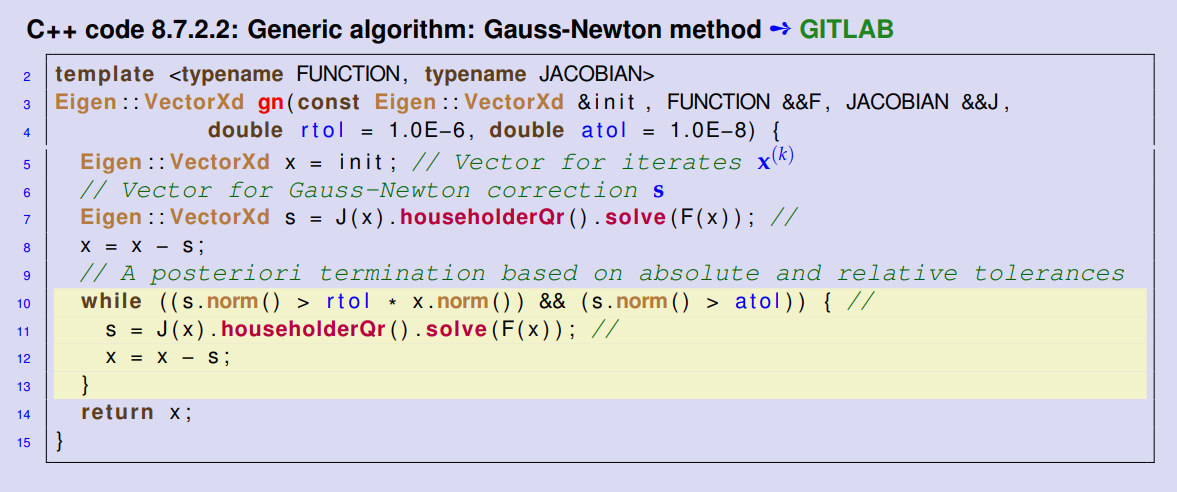
\includegraphics[width=1.0\linewidth]{CodeGaussNewtonMethod.png}
\end{figure}

\noindent As initial guess we choose $\mathbf{x}^{\left(0\right)} = \left[1,1,1,0.1\right]^{\mathsf{T}}$. The discussed norm $L_{\infty}$ is given in Eigen as $\\[2mm]$
\verb|lpNorm<Eigen::Infinity>()|
$\\[1mm]$

\noindent Which leads to the following code, which I copied from the master solution, as I could not come up with a solution on my own.
\begin{figure}[!hbt]
    \centering
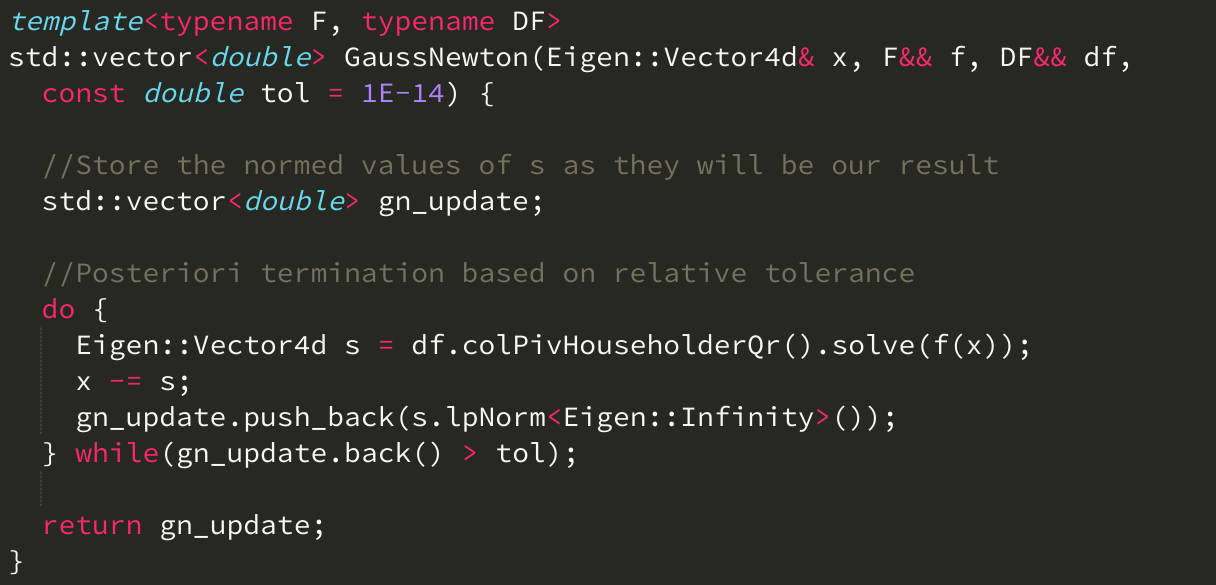
\includegraphics[width=0.9\linewidth]{8-11.d.png}
\end{figure}


\end{document}
